% Tracewall — evidence-backed IEEE draft (expanded)
% Claims only from EVIDENCE.md + eval/results/.
\documentclass[conference]{IEEEtran}

\usepackage[T1]{fontenc}
\usepackage[utf8]{inputenc}
\usepackage{amsmath,amssymb}
\usepackage{booktabs}
\usepackage{graphicx}
\usepackage{hyperref}
\usepackage{microtype}
\usepackage{xcolor}
\usepackage{listings}
\usepackage{cite}
\usepackage{tikz}
\usepackage{multirow}
\usepackage{array}
\usepackage{balance}
\usepackage{xurl}
\usetikzlibrary{arrows.meta,positioning,fit,calc}

\hypersetup{colorlinks=true,linkcolor=blue!50!black,urlcolor=blue!50!black,citecolor=blue!50!black}

\lstset{
  basicstyle=\ttfamily\scriptsize,
  breaklines=true,
  frame=single,
  backgroundcolor=\color{gray!6},
  rulecolor=\color{gray!40}
}

\title{Tracewall: Tool-Call Enforcement for AI Agents}

\author{
  \IEEEauthorblockN{beejak}
  \IEEEauthorblockA{
    \url{beejak@users.noreply.github.com}\\
    Draft preprint --- enforcement-only companion to \emph{agentwatch}\\
    Artifacts: \url{https://github.com/beejak/agentwatch-firewall}\\
    Evidence ledger: \path{paper/EVIDENCE.md} (through 2026-07-22)
  }
}

\begin{document}
\maketitle

\begin{abstract}
AI agents invoke tools that can move money, send email, and mutate shared state.
Prompt injection and capability misuse make those calls look legitimate on the wire.
We present \textbf{Tracewall}, a transport-agnostic \emph{tool-call PEP} (policy
enforcement point) with a single seam---
\texttt{Firewall.check}$\rightarrow$\texttt{FirewallVerdict}---that decides ALLOW or BLOCK
before a \emph{screened tool} side effect runs.
Tracewall does \emph{not} sit on the LLM chat stream to detect or neutralize jailbreaks;
after a prompt has already confused the agent, it gates the resulting tool calls.
The pipeline combines optional identity checks, a deterministic
YAML policy DSL (including call-tree context), a recovering multi-hop taint ledger, and an
optional semantic escalation tier (tier-0 content filtering is a noisy prior on tool-arg
text and never sole-BLOCKs). Fail-safe behavior is BLOCK on internal error.

On a frozen held-out corpus ($n{=}27$), the key-free path reaches deterministic integrated
recall $1.0$ (precision $\approx 0.929$, FPR $\approx 0.071$); tier-1 policy alone reaches
recall $1.0$ / FPR $0$. These numbers are a \emph{regression bar}, not adaptive proof.
AgentDojo defines multiple environment suites; we report a \emph{banking slice} only.
On that banking suite under DeepSeek with bill-preserving injections and a soft-block defense
(blocked tools become non-executing errors; the agent may continue), a \texttt{direct} attack
slice ($1{\times}4$) shows baseline ASR $1.0$ / utility $1.0$, falling to ASR $0.0$ / utility
$1.0$ under Tracewall. A cross-domain robustness matrix (workspace, HTTP, contagion, host,
identity; $18/18$) passes beyond banking-only probes. Full \texttt{Firewall.check} latency
on a mixed allow/block microbenchmark is mean $\approx 6.4$\,ms and p99 $\approx 9.8$\,ms
(deterministic backend, $n{=}400$). MCP stdio supports Content-Length framing and legacy
NDJSON, with brink tests that record successes and known limits.
We do \emph{not} claim $100\%$ detection on a small known-bad suite as a primary result,
nor sub-millisecond p99 latency versus GPU sentinels without a matched full-\texttt{check}
measurement, nor OS sandbox / on-disk scanning / SPIFFE as shipped Tracewall controls.
\end{abstract}

\begin{IEEEkeywords}
AI agents, tool-call firewall, prompt injection, AgentDojo, policy DSL, taint tracking, MCP
\end{IEEEkeywords}

\paragraph{TL;DR.}
One API decides ALLOW/BLOCK before \emph{tools} run---a tool-call PEP, not a chat
prompt scanner. YAML rules plus call trees catch exfil;
taint tracks contagion; soft-block keeps agents useful while stopping screened attacks.
Held-out recall $1.0$ is a regression bar. Soft-block AgentDojo banking \texttt{direct}
($1{\times}4$): ASR $0$, utility $1$. Cross-domain stress $18/18$. Mean \texttt{check}
$\approx 6.4$\,ms.

\paragraph{ELI5.}
Think of Tracewall as a bouncer for AI agents' \emph{tools}. Before an agent emails, pays a bill,
posts to chat, or uploads a file, the bouncer looks at \emph{which} tool, \emph{what}
arguments, and \emph{what it just did}. Stealing a secret and shipping it out? No.
Paying a normal bill? Yes. It is not a mind reader, not a chat-jailbreak scanner, and not an
OS sandbox---just a gate in front of dangerous tool actions after the model is already confused.

\section{Introduction}

Agent deployments add attack surfaces beyond single-turn chat:
(1)~\emph{input corruption}---instructions embedded in files or tool results
(e.g., MINJA-style memory/injection~\cite{minja});
(2)~\emph{capability abuse}---legitimate tools used for illegitimate goals
(email or money transfer after a sensitive read);
(3)~\emph{contagion}---taint flowing across agents or sessions via shared memory.

Content guardrails lack tool semantics. Wire gateways see destinations, not
\emph{why} a call was made. Dual-LLM interpreters redesign the agent stack~\cite{camel}.
Tracewall targets a narrower wedge: intercept tool calls, decide with policy and taint,
and keep evaluation honest (held-out ablation, brink limits, AgentDojo banking slices,
cross-domain stress). LLM compromise is assumed; the product is blast-radius control on
screened tools, not prompt neutralization.\footnote{%
\textbf{Scope.}
This paper is an evidence-backed description of Tracewall as a \emph{tool-call PEP}
(ALLOW/BLOCK before screened side effects)---not a chat-stream prompt scanner, OS sandbox,
or on-disk file scanner---with measured regression and eval discipline.
It \emph{proves} (narrowly) only claims marked VERIFIED in \path{paper/EVIDENCE.md}:
held-out corpus regression bars; MCP brink success$+$limits; firewall-only and
soft-block AgentDojo \emph{banking} slices where cited; a latency microbenchmark;
and the cross-domain stress matrix.
It does \emph{not} prove adaptive robustness; full AgentDojo coverage
(AgentDojo has multiple suites; we measured banking only);
production ZTA/SPIFFE identity; OS sandbox / kernel containment as shipped;
that Tracewall works if agents bypass the PEP;
superiority vs.\ GPU sentinels; or ``100\% detection'' marketing claims.}

\paragraph{Contributions.}
(1)~Stable enforcement seam with identity $\rightarrow$ content $\rightarrow$ YAML policy
$\rightarrow$ trust/taint $\rightarrow$ optional semantic judge $\rightarrow$ audit;
errors $\rightarrow$ BLOCK.
(2)~Deterministic policy pack (injection, exfil, destructive ops, workspace egress,
AgentDojo-shaped banking probes).
(3)~Multi-hop taint ledger with recovering trust.
(4)~Python guard and MCP stdio proxy (Content-Length $+$ NDJSON) with named profiles.
(5)~Evaluation discipline with an in-repo claim ledger and success vs.\ expected-limit rows.

\paragraph{Non-claims.}
We do not claim an observation-first OS or WatchTower branding; Hermes / graphify AST /
ruflo BFT / ClickHouse / SPIFFE CA as shipped product; GPU-sentinel latency comparisons
without matched methodology; or $100\%$ detection on a small known-bad suite as a primary
result. Tracewall is not a chat-stream prompt scanner (tier-0 is a noisy prior on tool args
and never sole BLOCK) and not an OS sandbox / on-disk file scanner.
Held-out tier-1 recall is not adaptive robustness. AgentDojo numbers are
banking-slice and model-specific (DeepSeek often refuses some jailbreaks); AgentDojo has
multiple suites---we do not claim full coverage.

\section{Related Work}

\paragraph{Injection and agent misuse.}
Indirect prompt injection remains a leading risk for tool-using LLMs.
MINJA~\cite{minja} showed high success via query-only memory poisoning; string filters
alone miss tool-level misuse after a sensitive read.

\paragraph{Firewalls, guardrails, and IFC.}
LlamaFirewall-style stacks combine classifiers with secondary LLM checks~\cite{llamafirewall}.
AgentSpec~\cite{agentspec} provides a runtime DSL without cross-session taint.
Wire gateways see destinations, not call trees. Dual-LLM IFC designs (e.g., CaMeL~\cite{camel})
redesign the agent stack; Tracewall instead inserts a single ALLOW/BLOCK seam before tools.

\paragraph{Benchmarks and taint.}
AgentDojo~\cite{agentdojo} scores utility and attack success under injection across
environments (banking, workspace, travel, \ldots). We treat it as an \emph{external bar}
and report only measured banking slices, plus a frozen corpus, MCP brink contracts, and a
non-banking robustness matrix. Classical taint is binary~\cite{newsome2005}; Tracewall uses
continuous trust/taint with hop/time decay. End-to-end MINJA vs.\ GPT-4 agents remains
unverified beyond synthetic ledger tests.

\section{Threat Model}

\textbf{Assumed:} the LLM may already be confused or compromised via prompts / tool results
(indirect injection). Tracewall does not claim to detect or neutralize that compromise in the
chat stream.
\textbf{In scope (tool-call blast radius):} misuse of available tools that pass through the PEP;
secret exfil via screened send/upload/http tools after a secret-reader in the call tree;
money-movement probes; destructive/remote-exec \texttt{bash} patterns when rules match;
capability / rate / allowlist abuse under \texttt{zta}/\texttt{paranoid}; single-agent
compromise that should raise taint when edges are recorded.
Tier-0 content filtering flags tool-arg text as a noisy prior and never sole-BLOCKs.
\textbf{Out of scope:} host / OS / kernel compromise; defeating or bypassing the PEP;
on-disk file content scanning; sandbox escape prevention (gVisor, landlock, seccomp, VM);
model-weight jailbreaks as the primary defense; chat-only compromise with no screened tool call;
adaptive paraphrases beyond the frozen held-out set unless measured; SPIFFE / continuous IdP
authentication as shipped; full AgentDojo (non-banking suites) unless measured.

\section{Design}

\subsection{Pipeline}
Figure~\ref{fig:arch} summarizes the enforcement path.

\begin{figure*}[!t]
\centering
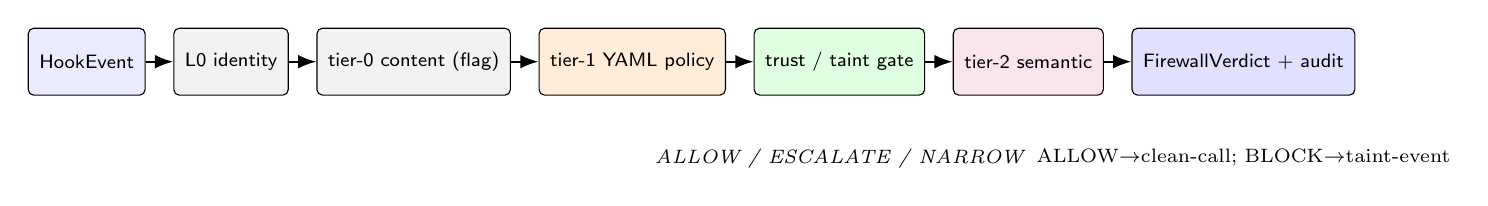
\begin{tikzpicture}[
  font=\scriptsize\sffamily,
  box/.style={draw, rounded corners=2pt, align=center, inner sep=4pt, minimum height=0.85cm},
  arr/.style={-{Latex}, thick}
]
\node[box, fill=blue!8] (hook) {HookEvent};
\node[box, right=0.35cm of hook, fill=gray!10] (l0) {L0 identity};
\node[box, right=0.35cm of l0, fill=gray!10] (t0) {tier-0 content (flag)};
\node[box, right=0.35cm of t0, fill=orange!15] (t1) {tier-1 YAML policy};
\node[box, right=0.35cm of t1, fill=green!12] (gate) {trust / taint gate};
\node[box, right=0.35cm of gate, fill=purple!10] (t2) {tier-2 semantic};
\node[box, right=0.35cm of t2, fill=blue!12] (ver) {FirewallVerdict + audit};
\draw[arr] (hook) -- (l0);
\draw[arr] (l0) -- (t0);
\draw[arr] (t0) -- (t1);
\draw[arr] (t1) -- (gate);
\draw[arr] (gate) -- (t2);
\draw[arr] (t2) -- (ver);
\node[below=0.55cm of gate, font=\scriptsize\itshape] {ALLOW / ESCALATE / NARROW};
\node[below=0.55cm of ver, align=center, font=\scriptsize]
  {ALLOW$\rightarrow$clean-call; BLOCK$\rightarrow$taint-event};
\end{tikzpicture}
\caption{Tracewall enforcement pipeline. Deterministic tiers are the fast path;
only escalations await the semantic judge. Internal errors fail safe to BLOCK.}
\label{fig:arch}
\end{figure*}

Verdict score is $0$ (bad) $\ldots$ $1$ (clean).
Context completeness records which signals were present on the event.

\subsection{Policy DSL}
Rules match tool name, argument operators, and call-tree constraints.
Argument operators include \texttt{regex}, \texttt{not\_in\_domain},
\texttt{host\_not\_in}, and \texttt{matches\_secret\_pattern}.
Call-tree predicates include \texttt{call\_tree\_contains}.
The token \texttt{\$\{ORG\_DOMAIN\}} expands from the environment variable
\texttt{TRACEWALL\_ORG\_DOMAINS}.
Match-level \texttt{rate\_exceeds} is an in-process sliding window
(not a distributed limiter). Profiles \textbf{zta}/\textbf{paranoid} load an
extra default-deny allowlist pack and may own the call tree in the MCP proxy.

\subsection{Taint / MTP}
A local SQLite ledger stores trust, taint, identity, and edges. Multi-hop taint
propagation solves a max-product fixed point with quarantine recovery.
Live \texttt{check()} updates trust on ALLOW/BLOCK; full contagion edges on MCP remain partial.

\subsection{Transports}
\begin{table}[!t]
\centering
\caption{Deployment placements.}
\label{tab:transports}
\small
\begin{tabular}{@{}p{0.30\columnwidth}p{0.62\columnwidth}@{}}
\toprule
Placement & Status \\
\midrule
Python guard & Shipped (\texttt{Firewall.check}) \\
MCP stdio proxy & Shipped; Content-Length $+$ NDJSON \\
GuardedToolNode & LangGraph-style pattern (no \texttt{langgraph} dep) \\
LangGraph / HTTP sidecar & Roadmap \\
\bottomrule
\end{tabular}
\end{table}
Profiles: \textbf{zta} (identity$+$caps, allowlists, proxy-owned call tree),
\textbf{paranoid}, \textbf{balanced} (lab default), \textbf{permissive}.

\section{Evaluation}

Primary numbers are from committed artifacts under \path{tracewall/eval/results/}
and \path{paper/EVIDENCE.md} (corpus/latency/AgentDojo live: 2026-07-19;
ZWSP/canonical closes and robustness $18/18$: 2026-07-21).

\subsection{Held-out corpus (key-free)}
Corpus \path{corpus_v0.1} test split, $n{=}27$ (13 malicious / 14 benign),
deterministic semantic backend.

\begin{table}[!t]
\centering
\caption{Held-out ablation (deterministic).}
\label{tab:heldout}
\begin{tabular}{@{}lccc@{}}
\toprule
Evaluator & Recall & Precision & FPR \\
\midrule
Tier-0 content & $0.0$ & $0.0$ & $0.143$ \\
Tier-1 policy & $1.0$ & $1.0$ & $0.0$ \\
Integrated & $1.0$ & $\approx0.929$ & $\approx0.071$ \\
Tier-2 semantic alone & $0.462$ & $0.857$ & $0.071$ \\
\bottomrule
\end{tabular}
\end{table}
\noindent\emph{Caveat:} not adaptive attacks; not AgentDojo.

\subsection{Latency}
Full \texttt{Firewall.check} on mixed allow/block events (deterministic backend,
warmup 40, $n{=}400$): mean $6.41$\,ms, p50 $6.82$\,ms, p95 $9.22$\,ms, p99 $9.82$\,ms
(\path{latency_check.json}). This is \emph{not} a claim of superiority vs.\ GPU
sentinels without matched end-to-end methodology.

\subsection{MCP brink}
Fourteen rows (9 success $+$ 5 expected\_limit): profiles block MINJA/exfil when configured;
limits include missing \texttt{\_meta}, permissive skipping the exfil pack, and unscanned
\texttt{tools/list}. Framing unit tests cover Content-Length encode/decode.

\subsection{Firewall-only AgentDojo-shaped stress}
Without an LLM, Tracewall blocks \texttt{send\_money} and \texttt{schedule\_transaction}
to the AgentDojo attacker IBAN and allows legitimate UK bill pay after \texttt{read\_file}.
Former bypasses (ZWSP-prefixed IBAN, wrong tool-name case) are closed as of 2026-07-21
via NFKC/ZWSP normalize and canonical tool names---now success rows, not expected\_limit.

\subsection{Cross-domain robustness (non-banking)}
Beyond banking, a firewall-only matrix covers workspace messaging, HTTP POST, upload,
memory contagion, host write paths, and identity/caps
($16$ success $+\,2$ expected\_limit $=\,18/18$ in \path{robustness_stress.json}).
Successes include blocking Slack-shaped \texttt{send\_message}, \texttt{http\_post}, and
\texttt{upload} after secret reads, identity denials when required, ZWSP IBAN normalize,
and PascalCase tool aliases after canonicalization.
Tracked expected limits: unknown tool names and unscanned MCP \texttt{tools/list}.
This is still not adaptive attack proof---it widens the \emph{domain} surface under test.

\subsection{AgentDojo live (DeepSeek)}
\textbf{Setup:} banking; bill-preserving injections; benchmark system prompt (eval-only);
model \texttt{deepseek-chat}. Defense default is \emph{soft-block} (rewrite blocked tool
names so execution yields an error without aborting the agent).

\begin{table}[!t]
\centering
\caption{AgentDojo banking live (DeepSeek, bill-preserving). ASR $=$ injection goal met.
Abort $=$ hard BLOCK; soft $=$ rewrite blocked tool to a non-executing error.}
\label{tab:adojo}
\small
\begin{tabular}{@{}llcrr@{}}
\toprule
Attack / slice & Arm & ASR & Utility \\
\midrule
imp.\ instr.\ ($1{\times}1$) & base / def. & $0.0$ / $0.0$ & $1.0$ / $1.0$ \\
ignore prev.\ ($1{\times}1$) & base / def. & $0.0$ / $0.0$ & $1.0$ / $1.0$ \\
direct ($1{\times}1$, abort) & base $\rightarrow$ def. & $1.0\rightarrow0.0$ & $1.0\rightarrow1.0$ \\
direct ($1{\times}4$, abort) & base $\rightarrow$ def. & $1.0\rightarrow0.0$ & $1.0\rightarrow0.25$ \\
direct ($1{\times}4$, soft) & base $\rightarrow$ def. & $1.0\rightarrow0.0$ & $1.0\rightarrow1.0$ \\
\bottomrule
\end{tabular}
\end{table}

Under \texttt{direct}, baseline ASR is $1.0$; Tracewall drives ASR to $0.0$.
Abort-on-BLOCK taxed utility on the $1{\times}4$ expand ($0.25$); \textbf{soft-block}
keeps utility at $1.0$ while still preventing the injection goal.
Jailbreaks with baseline ASR $0$ are model refusals---not credited as Tracewall wins.

\section{Making it more robust (roadmap)}
Concrete next bars (not yet VERIFIED as paper wins):
AgentDojo workspace/travel suites; signed workload identity;
full LangGraph package integration / HTTP sidecar PEP;
org allowlists instead of attacker-IBAN probes; live contagion edges on MCP;
adaptive paraphrase corpus; distributed (cluster) rate limits.
(ZWSP/NFKC IBAN normalize and canonical tool-name aliases are shipped.)

\section{Limitations}

Tracewall is a \emph{tool-call PEP}, not a chat-stream scanner or OS sandbox; PEP bypass,
unknown tools, host escape, and chat-only jailbreaks without a screened tool call remain open.
Contagion on live MCP edges is incomplete. Semantic LLM is optional and non-gating.
AgentDojo defines multiple suites; our coverage remains a \emph{banking} slice.
Attacker-IBAN rules are eval-aligned probes; production needs org allowlists.
Latency is a single-host microbenchmark.
Unknown tool names and unscanned MCP \texttt{tools/list} remain expected limits
(ZWSP IBAN and PascalCase aliases are closed).
No SPIFFE / signed workload identity (ledger register only).

\section{Conclusion}

Tracewall is a practical \emph{tool-call PEP}: deterministic policy and taint-aware routing
behind one API, with Python and MCP transports. It contains screened tool side effects after
LLM compromise---not chat-stream neutralization or OS sandboxing. Evidence favors held-out
ablation, brink honesty, cross-domain stress, measured \texttt{check} latency, and AgentDojo
\emph{banking} slices where the model attempts the attack---so ALLOW/BLOCK can be attributed
to the firewall rather than to refusal.

\section*{Artifacts}
\begin{itemize}
\setlength{\itemsep}{1pt}
\setlength{\parsep}{0pt}
\setlength{\parskip}{0pt}
\item \path{corpus_v0.1_test_deterministic.json}
\item \path{mcp_brink.json}
\item \path{adojo_stress.json}
\item \path{latency_check.json}
\item \path{robustness_stress.json}
\item \path{paper/EVIDENCE.md}
\end{itemize}

\balance
\begin{thebibliography}{00}
\bibitem{minja} C.~Zheng et al., ``MINJA: Memory Injection Attack,'' arXiv:2503.03704, 2025.
\bibitem{agentspec} Z.~Wang et al., ``AgentSpec,'' arXiv:2503.18666, 2025.
\bibitem{agentdojo} E.~Debenedetti et al., ``AgentDojo: A Dynamic Environment to Evaluate
Prompt Injection Attacks and Defenses for LLM Agents,'' 2024.
\bibitem{llamafirewall} Meta, ``LlamaFirewall,'' arXiv:2505.03574, 2025.
\bibitem{camel} CaMeL / dual-LLM IFC agent designs (see contemporary agent security literature).
\bibitem{newsome2005} J.~Newsome and D.~Song, ``Dynamic Taint Analysis for Automatic Detection,
Analysis, and Signature Generation of Exploits on Commodity Software,'' NDSS, 2005.
\end{thebibliography}

\end{document}
